\section{The RationalGRL Methodology and Tool}
\label{sect:methodology}

In previous sections, we have shown how the RationalGRL framework can capture stakeholder discussions, and how interactions between two types of reasoning, practical reasoning and goal modeling, leads to two interlinked models, RationalGRL and GRL models. In this section we clarify how practitioners can actually use the RationalGRL framework by proposing a methodology\footnote{The methodology presented here was first presented at the 2017 iStar workshop \cite{ghanavatiMethodology}.} (\textbf{requirement 4}) and discussing a prototype RationalGRL tool (\textbf{requirement 5}).

\subsection{RationalGRL Methodology}
\label{sect:methodology} 

We propose the methodology shown in Figure~\ref{fig:rationalgrl-methodology} to develop a (Rational)GRL model. %Here we assume that the initial GRL models have been created based on the requirements specification documents and the discussions of the stakeholders. The rest of the steps are as follows:

\begin{figure*}[ht]
\centering
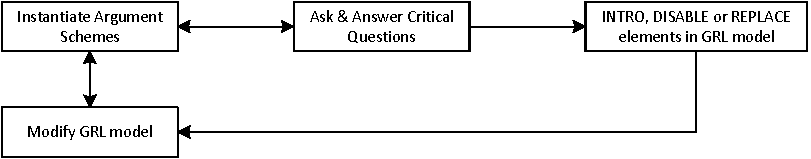
\includegraphics{img/methodology.pdf}
\caption{The RationalGRL Methodology}
\label{fig:rationalgrl-methodology}
\end{figure*}

\textbf{(1) Instantiate Argument Schemes (AS)} -- We start with the list of argument schemes (Table~\ref{table:argument-schemes}). Whilst discussing the requirements, we select schemes from the list and instantiate them to form arguments for GRL model elements. In this way we build or modify the GRL model by introducing new GRL elements (\textsf{INTRO}). Note that it is also possible to start modifying an existing GRL model which was not built using the RationalGRL methodology: each GRL element corresponds to an argument (i.e. an instantiated scheme), so it is possible to instantiate argument schemes based on an existing GRL model. 

\textbf{(2) Answer Critical Questions (CQs)} -- After building or modifying the initial GRL model, we ask the relevant critical questions. Because each element in the GRL model corresponds to an instantiated scheme, we can look at Table~\ref{table:argument-schemes}) to see which questions are relevant given our GRL model. 

\textbf{(3) Decide on Intentional Elements and their Relationships} -- By answering a critical question, one of three operations are performed on the GRL model: \textsf{INTRO}, \textsf{DISABLE} or \textsf{REPLACE}. Any of these operations impact the arguments and corresponding GRL intentional elements, modifying the initial GRL model into a RationalGRL model. After these modifications, we can keep on asking critical questions (e.g. about elements that were introduced by previously answering a critical question) until we are satisfied with our model.   

\textbf{(4) Modify GRL Models} -- In this step, we modify the regular GRL model based on the RationalGRL model of step (3). That is, one of the following situation can happen with respect to the initial GRL model: 1) a new intentional element or a new link is introduced; 2) an existing intentional element or an existing link gets disabled (removed) from the model; or 3) an existing intentional element or link is replaced by a new one. This results in a new, modified GRL model, which can be used as the basis for another cycle of the methodology. 

We can continue these four steps until there is no more intentional element or link to analyze or we reach a satisfactory model. In the next section, we will give an example of how our tool can be used together with the methodology to build a GRL model.  

\subsection{The RationalGRL Tool}
\label{sect:tool}

An important requirement of our framework is that it has tool support. This is for various reasons: i) although there are various approaches attempting to combine goal modeling with argumentation, there does not yet exist any tool support (see Section~\ref{sect:discussion}), ii) it allows us to do user tests in future research, exploring the difference between GRL and RationalGRL, iii) tool support is an excellent verification to ensure our formal framework and algorithms actually work, iv) having a light-weight web-based version of GRL is useful for the community in general.

GRL has a well-documented and well-maintained tool called jUCMNav~\cite{jUCMNav}. This tool is an extension to Eclipse. Although it is a rich tool with many features, it is implemented as an Eclipse plugin. We have experienced on various occasions that setting this up properly can take up a significant time of experiments, leaving less time for actual modeling.

Our formalization of GRL is very much in line with the way in which GRL models are represented in the open-source Eclipse-based tool jUCMNav.\footnote{See \url{http://jucmnav.softwareengineering.ca/foswiki/ProjetSEG}} By keeping our formalization in line with this tool, we simplify the translation step from models in the RationalGRL tool to models in the jUCMNav tool.

In this section we present our web-based prototype of RationalGRL. It can be accessed from:
\begin{quote}
\url{http://www.rationalgrl.com}
\end{quote}

The tool is written in Javascript, and runs on all modern browsers. The tool is open-source, and the source can be accessed from:
\begin{quote}
\url{http://www.github.com/marcvanzee/RationalGRL}
\end{quote}

In this section we briefly highlight some features of the language, and we explain some of its current limitations.

\todo{all}{marc}{Explain figures in Appendix~\ref{sect:tool-screenshots}}